\section{W3: Risk Management}

\textbf{Risk vs Uncertainty}: Risk is uncertainty that has a measurable impact. Uncertainty is the lack of certainty about an event/outcome.

\textbf{Understand the Risk Management Process.}

% understand how to
    \textbf{Plan risk management activities.}

    A RMP (Risk Management Plan) documents the procedures for managing risks. It includes: methodology, roles and responsibilities, budget and schedule, risk categories, risk probability and impact, tracking, risk documentation, contingency plans, fallback plans.

    Kinds of risks: project, product and business.

    \textbf{Identify risks.}

    Pondering, interviewing, brainstoming, checklists, Delphi technique (a group of experts anonymously contribute their opinions on a topic, and then update their responses until a consensus is reached), SWOT analysis (case study) for Strengths, Weaknesses, Opportunities, Threats.

    \textbf{Analyze and assess risks.}
    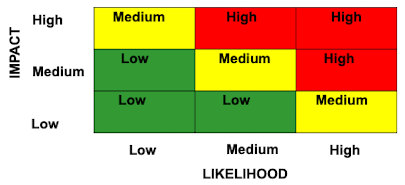
\includegraphics[width=\linewidth]{figs/SCR-20240605-sqml.png}
    Qualitative: Risk exposure = probability of occurrence * impact of occurrence.
    Quantitative: decision tree analysis, simulation, sensitivity analysis.


    \textbf{Respond to risks (risk strategies)}


    \textbf{Monitor and control risks.}

% topics include

    \textbf{Monitor and Control Risks.}

    \textbf{Risk Management in Agile (factors specific to Agile and Scrum).}

    \textbf{SWOT Analysis.}
